\section{Abstract *}\label{abstract}

The rubiks cube is perhap's the world's most famous puzzle, or certainly
an iconic one at that. It is widely believed to have been first
concieved by Hungarian Professor of Architecture Erno Rubik in an
attempt to demonstrate 3-Dimensional Design, in Particular 3-Dimensional
motion, to his students. He was also the first to come up with a
solution to the puzzle (conceived after one month of inventing). Since
it's rise to popularity, it has entertained the minds of many people,
some of whom were mathematicians. It's first rigorous mathematical
analysis was done by British-American Mathemetician David Singmaster,
though solutions were known to a number of mathematicians by then (Such
as J.H. Conway and Roger Penrose)
{[}https://www.youtube.com/watch?v=DtYr\_3h0Ubw{]}.

In this project we discuss the motivation to consider the Rubiks cube as
a mathematical object, It's modelling, and as such the results that
arise from it's modelling for instance the contruction of the Illegal
Rubik's Cube Group, the subset of which is the Legal Rubik's Cube Group,
which can be seen as a consequence of the fundamental theorems of
Cubology (according to sources this varies). After the derivation and
construction of the model with which we are working with we look into
how to solve the rubik's cube. Note we are essentially considering only
the 3x3x3 cube.

\section{Attempting to Understand the Cube
*}\label{attempting-to-understand-the-cube}

What is it that we are essentially trying to understand with the cube as
it is presented? Well when we consider the appearance of the Rubik's
cube Rubiks cube group (How we derive the group for modeling the cube),
For starters take into account that the Rubik's cube is composed of 26
mechanical pieces (called cubies) held together, Furthermore we note we
have - 8 corner cubies - 12 edge cubies - 6 Center cubies -
\(9 \times 6 = 54\) Facets (small faces) (Insert a picture of the three
type of cubies -- ?) Note that regardless of motion the 6 center cubes
stay fixed. We start counting the the possible configurations of the
cubes.

\subsection{Combinatorics *}\label{combinatorics}

{[}https://www.sfu.ca/\textasciitilde jtmulhol/math302/puzzles-rc-cubology.html,
Daniels' project, Bandelow{]}

We count the total number of configurations given the established types
of cubies - There are 8 cubies, and hence 8! ways of arranging them -
There are 12 edge cubies, and hence 12! ways of arranging those - There
are 3 colors per each corner cubie, 3\^{}\{8\} ways of arranging those -
There are 2 colors per each edge cubie, 2\^{}\{12\} ways of arranging
those

Multiplying these numbers together we get
\(8!\cdot 12! \cdot 3^{8} \cdot 2^{12} = 519024039293878272000\) This
consists of the illegal arrangement of the elements in the Rubik's cube
group. We will note how to construct the legal rubix cube group as a
subset of this.

We note that the rubik's cube group is a subset of \(S_{54}\) as it
provides \(54\) facets with permutations.

\subsection{Construction of the illegal Rubik cube
group}\label{construction-of-the-illegal-rubik-cube-group}

{[}Daniel's project{]}

\subsubsection{Preliminaries}\label{preliminaries}

\begin{enumerate}
\def\labelenumi{\arabic{enumi}.}
\item
  Direct products (External direct product)
\item
  Semi-direct products:
\end{enumerate}

A Weaker version of an inner product where only one of the subgroups has
to be normal

\textbf{Theorem} Let \(G\) be a group with subgroups \(H\) and \(K\)
such that

\begin{enumerate}
\def\labelenumi{(\arabic{enumi})}
\item
  \(G = NH\)
\item
  \(N \cap H = e\)
\item
  \(N \triangleleft K\) {[}keith conrad, semidirect products{]}
\end{enumerate}

\begin{enumerate}
\def\labelenumi{\arabic{enumi}.}
\setcounter{enumi}{2}
\tightlist
\item
  Wreath products:
\end{enumerate}

The wreath products of two groups G and H is constructed by:

\begin{enumerate}
\def\labelenumi{\arabic{enumi}.}
\item
  Write H as a permutation on n items
\item
  Make n copies of the group G. \((G^n)\)
\item
  H acts on the copies of G by permuting the elements.
\end{enumerate}

The wreath product of G by H is a semi-direct product of a direct
products of n copies of G by H.

The wreath product permutes the factors of G according to the action h
on X. So if \(x \in G\), then the wreath product would take components
of G and shuffle them around according to the action h on the set X.

\subsubsection{Example of a wreath product:
*}\label{example-of-a-wreath-product}

\(G = \mathbb Z_2\), \(H = S_3\), and \(X = \{1,2,3\}\). The wreath
product of G by H is \(\mathbb Z_2^3 \wr S_3\)

So the elements of \(\mathbb Z_2^3 \wr S_3\) are:

\[\{(0,0,0)\sigma,(1,0,0)\sigma,(0,1,0)\sigma,(0,0,1)\sigma,(1,1,0)\sigma,(0,1,1)\sigma,(1,0,1)\sigma,(1,1,1)\sigma\}\]

Where \(\sigma \in S_3\)

\begin{enumerate}
\def\labelenumi{\arabic{enumi}.}
\item
  \(1/2\) of the permutations of the edges and corners are possible
  since we require even permutations?
\item
  \(1/2\) of the orientations of the edges are possible since the number
  of flipped edges has to be even.
\item
  \(1/3\) of the corner orientations are possible. (Fundamental theorem
  of cubology b)
\end{enumerate}

\subsection{Position Vectors}\label{position-vectors}

For a given configuration of a Rubik's Cube there exists a \(4\) tuple
\((\rho, \sigma, v, w))\) where \(\rho \in S_8, \sigma \in S_{12}\)
describe the permutations of the cubies and
\(v \in \mathbb Z_3^8, w \in \mathbb Z_2^{12}\) describe the
orientations of the cubies.

\subsection{Notation *}\label{notation}

The most popular set of notations are from Singmaster and we shall adopt
them here, note that we label the face with respect to it lying flat on
a plane and one is facing front face)

\begin{itemize}
\tightlist
\item
  Let \(U\) denote the upward (top) face.
\item
  Let \(F\) denote the front face.
\item
  Let \(L\) denote the left face.
\item
  Let \(R\) denote the right face.
\item
  Let \(B\) denote the back face.
\item
  Let \(D\) denote the downward (bottom) face (insert picture here)
\end{itemize}

The capital letter represent a \(90\degree\) turn clockwise facing that
face. The inverse of each move would be the \(90\degree\) rotation of
the face counter-clockwise (denoted by a \(M^{-1}\) in our adaptation
where \(M\) \in \{F,L,U,D,R,B \}\$).

\emph{Example}: The combunation of moves \(UFR\) denotes a move
consisting of \(90\degree\) clowise turns done to the top, then front,
and then the right face. The inverse of this is \(R^{-1}F^{-1}U^{-1})\).

\subsection{The Rubiks cube Group *}\label{the-rubiks-cube-group}

{[}Daniels project, Singmaster Notes, Bandelow{]}

Recall, that the rubiks cube consists of \(54\) facets, and the entire
set of arrangements of the rubiks cube can be thought of as permutations
of these 54 facets. Hence we can denote
\(G = \langle F,L,U,D,R,B\rangle \subset S_{54}\) as the called rubik's
cube group.

Now note that not all arrangments of the permutations would lead to the
valid arrangements of a rubik's cube, this group includes all cubes that
can be taken apart and put together (the illegal rubiks' cube group),
e.g.~not pieces can alternate between being either corner and edge
cubies, and those that can be reached by applying moves on the cube (the
legal rubik's cube group).

Note that it is the case that the corner facets can be modelled as the
cyclic group of 3 elements \(C_{3}\) and since there are 8 of theese we
note it is the corss product of \(C_{3}\) eight times.

Now, the possible arrangements of the corner cubes can be described
using \(S_{8}\) (since we are permuting those), which allows the
postions of all the corner facets on the Rubik's Cube to be described as
the group \(C_{3}^{8} \wr S_{8}\).

By a similar argument we see that the position of all the edge facets on
the Rubik's Cube can be described by the group \(C_{2}^{2} \wr s_{12}\).

\subsubsection{Definition of an illegal rubik's group
*}\label{definition-of-an-illegal-rubiks-group}

Unlike the legal Rubik's cube group, the Illegal Rubik's Cube Group
allows the solver to take the cube apart and rearrange the facets.
However, we also notice that some orientations still will not be
physically possible on the cube. We also notice that the Rubik's cube
group is a subgroup of the illegal rubik's cube group.

So from the description of the corner and edge cubes, we can see that
the illegal rubik's cube group is
\(I = (C^{12}_2 \wr S_{12}) \times (C^8_3 \wr S_8)\).

\subsection{Construction of the legal Rubix cube group
*}\label{construction-of-the-legal-rubix-cube-group}

{[}https://www.sfu.ca/\textasciitilde jtmulhol/math302/puzzles-rc-cubology.html{]}
\^{} Talk about this after the fundamental theorem of cubology?
Attempting to derive the legal rubik's cube group requires the
construction of the Fundamential Theorem of Cubology, and the second
fundamental theorem of cubology

\subsubsection{Rubiks Specific Theorems
*}\label{rubiks-specific-theorems}

In this section, we will state the main theorem of our topic and any
lemmas required to understand the main theorem.

\subsection{Theorem on Parity}\label{theorem-on-parity}

Permutations can also be described in terms of their parity. Any length
n cycle of a permutation can be expressed as the product of 2-cycles.

The cube always has even parity, or an even number of cubies exchanged
from the starting position.

\subsection{Main Theorem: Fundamental Theorem of Cubology
*}\label{main-theorem-fundamental-theorem-of-cubology}

A move sequence is possible if and only if the following three
conditions are satisfied, we also state the group theoretic formulation:

Note we are considering the following defintion of a postion of a facet
of a cube: A position vector
\((\rho,\sigma,v,w) \in S_{8} \times S_{12} \times C_{3}^{8} \times C_{2}^{12}\)
- The permutation of the corner cubies has the same parity as the
permutation of the edge cubies \(\Leftrightarrow\)
\[\text{sign}(\rho) = \text{sign}(\sigma)\]

\begin{itemize}
\tightlist
\item
  The number of corners that are twisted clockwise is equal to the
  number that are twisted counterclockwise modulo \(3\) (meaning
  remaining corners twisted in the same direction occur in threes).
  \(\Leftrightarrow\)
  \[v_{1} + v_{2} +\dots +v_{8} = 0 (\text{mod } 3)\]
\item
  The number of flipped edges is even. \(\Leftrightarrow\)
  \[w_{1} + w_{2} +\dots +w_{12} = 0 (\text{mod } 2)\]
\end{itemize}

\subsection{Summarized proof ?}\label{summarized-proof}

The first thing to show is that the three conditions are necessary, that
is, they hold for any legal configuration. To do this we just need to
show that if the conditions are satisfied for a configuration, then they
also hold for the configuration obtained from it by twising one of the
six faces. This involves just looking at the six cases individually.

Next we would need to show that if we had a configuration that satisfies
the three conditions then the puzzle is solvable. Here is where our four
basic moves come in handy. Let's recall them here for convenience.

Since the corner and edge permutations have the same parity we can
assume they are both even (otherwise twist any random face 90 degrees
since this would multiply each by a 4-cycle which is odd). Since the
corner permuation is even it is a product of 3-cycles, therefore the
corners can be solved using 3-cycles. (We have a 3-cycle move that can
be modified to cycle any 3 corner cubies on the puzzle.) Similarly, the
edge permutation is even and can be solved using 3-cycles.

Now all cubies are in their correct cubicles. We now have to orient them
to solve the puzzle. Condition (b) says that the number of clockwise
corner twists is equal to the number of counterclockwise corner twists
modulo 3 . So first twist any cw, ccw pairs into their solved positions.
The result will be that all remaining corner twists will occur in
triples: 3cw or 3ccw. These can be solved using our pairwise corner
twisting moves. Finally, condition (c) says an even number of edges will
be flipped. Luckily we have a move that will flip them in pairs.
Therefore the puzzle can be solved.

\subsection{Second Fundamental Theorem of Cubology
*}\label{second-fundamental-theorem-of-cubology}

An operation of the cube is possible if and only if the following are
satisfied: - The total number of edge and corner cycles of even length
is even. - The number of corner cycles twisted right is equal to the
number of corner cycles twisted left (up to modulo 3). - There is an
even number of reorienting edge cycles.

\subsection{Ultimate Result *}\label{ultimate-result}

We can now effectively conclude that

\(RC \approx (C_{3}^{7} \wr S_{8}) \times (C_{2}^{11} \wr S_{12})\)

\section{Algorithms}\label{algorithms}

\subsection{A Modified version of the Bottom Up
Approach}\label{a-modified-version-of-the-bottom-up-approach}

\subsection{Bottom Up Algorithm}\label{bottom-up-algorithm}

A general and quite commonly used Rubik's Cube Solution is solving a
cube layer by layer:

\begin{itemize}
\tightlist
\item
  Pick a face
\item
  solve for the edges
\item
  then solve corners
\item
  Go down to the next layer solve for the edges (sisnce there are no
  corners)
\item
  Go to the final layer, solve for the edge and solve corners
\end{itemize}

\section{Section 3}\label{section-3}

In this section we will present a summarized proof of our main theorem,
namely, the Fundamental Theorem of Cubology.

\subsection{Summarized Proof of the Fundamental Theorem of Cubology *
(redundant)}\label{summarized-proof-of-the-fundamental-theorem-of-cubology-redundant}

\begin{figure}
\centering
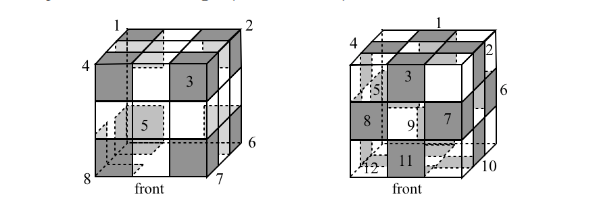
\includegraphics{Screenshot from 2024-03-08 10-56-32.png}
\caption{The numbering in question:}
\end{figure}

Begin with a cube in any configuration. We add a ``+'' mark to each
cubicle, where each cubicle can only have 1 of these ``+'' marks to 1 of
their facets. There are a number of ways for doing this, so we will call
the facet we mark for each cubicle the ``primary facet''.

For example:

\begin{figure}
\centering
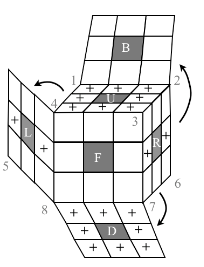
\includegraphics{Screenshot from 2024-03-08 11-03-50.png}
\caption{An example of an orientation:}
\end{figure}

Then, we mark the remaining facets based on the primary facet. For an
edge cubie, mark the sticker with a 0 if it is the primary facet, and
mark the other sticker on the same cubie with a 1. For a corner cubie,
mark the sticker in the primary facet with a 0 , and mark the other two
stickers with 1 and 2.

\begin{figure}
\centering
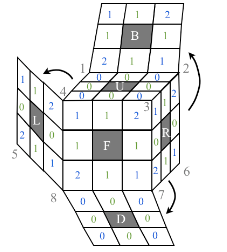
\includegraphics{Screenshot from 2024-03-08 11-07-22.png}
\caption{Updated marking with numbers of the previous orientation:}
\end{figure}

We notice that we can use a 4-tuple, \((\rho, \sigma,v,w)\) to describe
any configuration of the cube. Where \(\rho \in S_8\),
\(\sigma \in S_{12}\), \(v \in C_8^{12}\) and \(w \in C_2^{12}\).

\section{Section 4 *}\label{section-4}

In this section we demonstrate which cubes are solvable and which ones
aren't by applying the Fundamental Theorem of Cubology

The types of solvable cubes

Types of non-solvable cubes and explanation
https://speedcubeshop.ca/a/blog/unsolvable-rubiks-cubes

\#\# Corner twist

A singular twisted corner is an impossible case to get on
\(3 \times 3\).

As previously stated, the cube always has even parity. However, a corner
twist is an odd permutation.

\begin{figure}
\centering
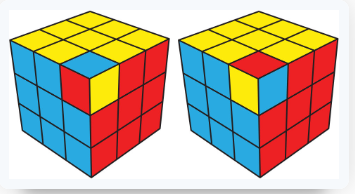
\includegraphics{Screenshot from 2024-03-24 08-41-47-1.png}
\caption{Example of a corner twist}
\end{figure}

\#\# Swapped pieces

Two edge pieces cannot be swapped, either adjacently or opposite on a
\(3 \times 3\) Rubik's cube. The same can be said for two corner pieces.

Similar to the corner twist, swapped pieces produces odd permutations.

\begin{figure}
\centering
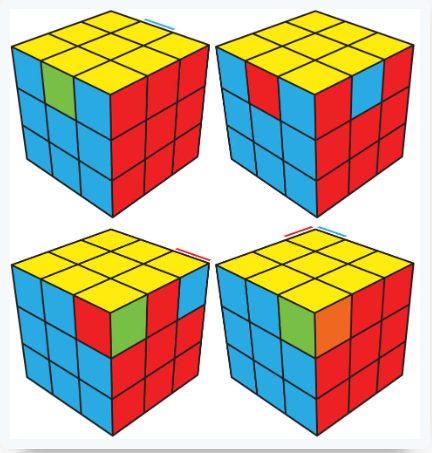
\includegraphics{Screenshot from 2024-03-24 08-42-10-1.png}
\caption{Examples of swapped pieces}
\end{figure}

\subsection{Exactly one edge cubie is flipped
*}\label{exactly-one-edge-cubie-is-flipped}

\begin{figure}
\centering
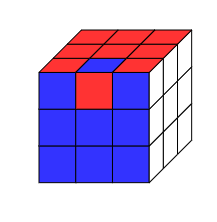
\includegraphics{Screenshot from 2024-03-26 11-14-42-1.png}
\caption{Example of cube with one edge flipped}
\end{figure}

\section{Section 5}\label{section-5}

In this section we discuss how the Fundamental Theorem of Cubology
relates to the content covered in MATH 4GR3.

\begin{itemize}
\tightlist
\item
  Conjugation as a group action on the Rubik's Cube
\end{itemize}

\section{Section 6 *}\label{section-6}

In this section we list all of our references.

Daniels, L. (2014). Group Theory and the Rubik's Cube.
http://math.fon.rs/files/DanielsProject58.pdf
